\documentclass{article}

\usepackage{float}
\usepackage[version=3]{mhchem} % Package for chemical equation typesetting
\usepackage{siunitx} % Provides the \SI{}{} and \si{} command for typesetting SI units
\usepackage{graphicx} % Required for the inclusion of images
\usepackage{natbib} % Required to change bibliography style to APA
\usepackage{amsmath} % Required for some math elements
\usepackage{subfigure}
\usepackage{listings}

\setlength\parindent{0pt} % Removes all indentation from paragraphs

\renewcommand{\labelenumi}{\alph{enumi}.} % Make numbering in the enumerate environment by letter rather than number (e.g. section 6)

%\usepackage{times} % Uncomment to use the Times New Roman font

%----------------------------------------------------------------------------------------
%	DOCUMENT INFORMATION
%----------------------------------------------------------------------------------------

\title{Computer Vision \\ Lab3 \\ ECE5470} % Title

\author{Yuqing Shou \\ ys895@cornell.edu} % Author name

\date{\ 9/27/2018} % Date for the report


\begin{document}


\maketitle % Insert the title, author and date

\begin{center}
\begin{tabular}{l r}
Instructor: & Professor Reeves, A % Instructor/supervisor
\end{tabular}
\end{center}

% If you wish to include an abstract, uncomment the lines below
% \begin{abstract}
% Abstract text
% \end{abstract}

\newpage

%\begin{center}\ce{2 Mg + O2 -> 2 MgO}\end{center}

% If you have more than one objective, uncomment the below:
%\begin{description}
%\item[First Objective] \hfill \\
%Objective 1 text
%\item[Second Objective] \hfill \\
%Objective 2 text
%\end{description}

\section*{Section2 Peakiness Detection}
The output pictures are shown in the below, it shows that the Peakiness algorithm faces a lot of disadvantages in the field of
image thresholding. The conclusion is below:
The Peakiness Algorithm has the advantages that it can threshold the image pretty easy without those time consuming operation doing on the image, however, it is also one of the disadvantages in a different view.
From the Figure2, we get that when d=6 and d=5, there is a big gape between the quality of the images.When d=6 the pixels in low part of the object disappeared, when d=6, the low part of the objects become too dark to be observed, it reveals one of the most important disadvantages of Peakiness Algorithm: people have to exert time to find the most suitable threshold, which is time consuming.
\par
\vspace{3mm}
From the Figure 3,4,5, we can get that the Peakiness Algorithm's threshold influenced the clearness of images significantly, different pictures shows different suitable thresholds. Some of pictures shows that the thresholds also influence the people's perception.

\begin{figure}[H]
\centering
\subfigure[d=5.]{
\begin{minipage}[t]{0.25\linewidth}
\centering
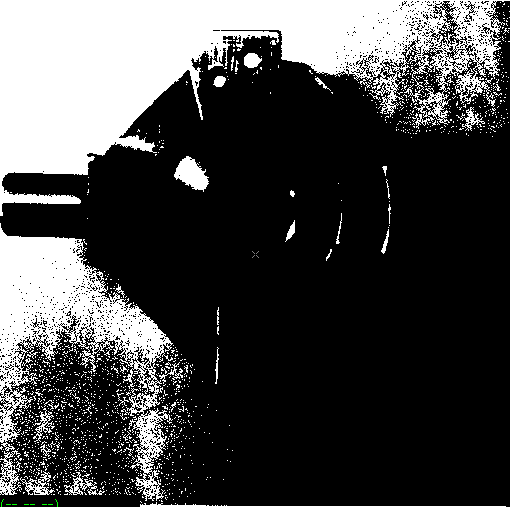
\includegraphics[width=3cm]{d=5}
%\caption{fig1}
\end{minipage}%
}%
\subfigure[d=6.]{
\begin{minipage}[t]{0.25\linewidth}
\centering
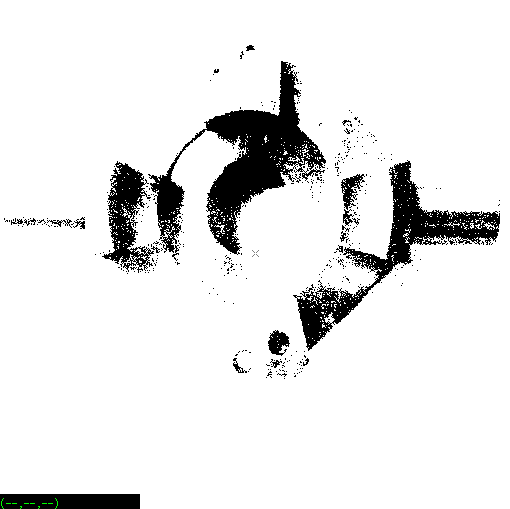
\includegraphics[width=3cm]{d=6}
%\caption{fig2}
\end{minipage}%
}%

\subfigure[d=7.]{
\begin{minipage}[t]{0.25\linewidth}
\centering
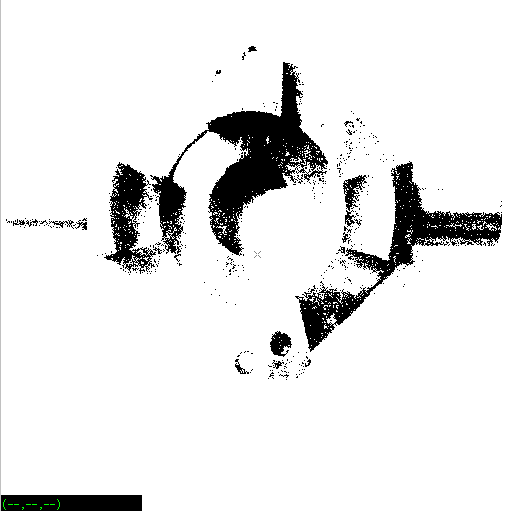
\includegraphics[width=3cm]{d=7}
%\caption{fig2}
\end{minipage}
}%
\subfigure[d=10.]{
\begin{minipage}[t]{0.25\linewidth}
\centering
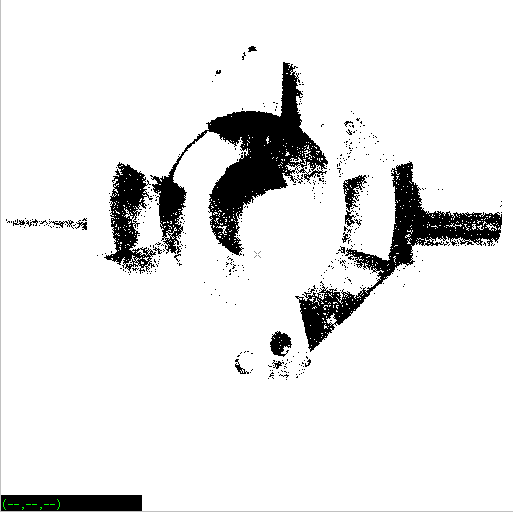
\includegraphics[width=3cm]{d=10}
%\caption{fig2}
\end{minipage}
}%
\centering
\caption{ Picture of mp}
\end{figure}
\begin{figure}[H]
\centering
\subfigure[d=6.]{
\begin{minipage}[t]{0.25\linewidth}
\centering
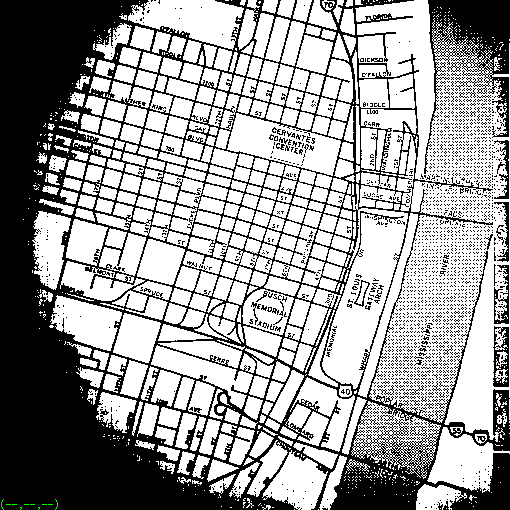
\includegraphics[width=3cm]{map_d=6}
%\caption{fig1}
\end{minipage}%
}%
\subfigure[d=10.]{
\begin{minipage}[t]{0.25\linewidth}
\centering
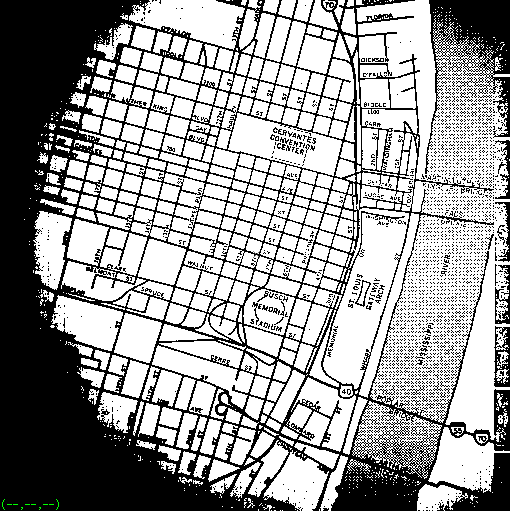
\includegraphics[width=3cm]{map_d=10}
%\caption{fig2}
\end{minipage}%
}%

\subfigure[d=30.]{
\begin{minipage}[t]{0.25\linewidth}
\centering
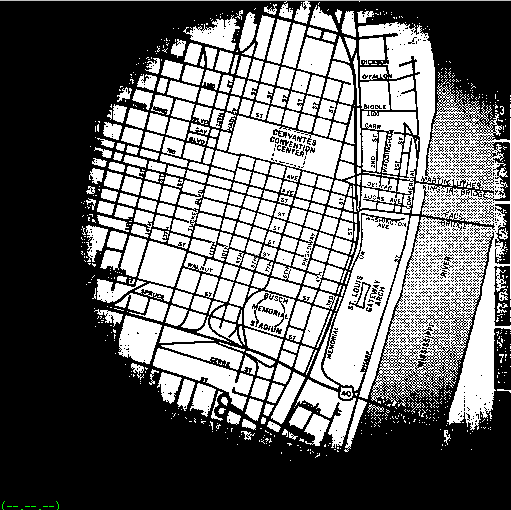
\includegraphics[width=3cm]{map_d=30}
%\caption{fig2}
\end{minipage}
}%
\centering
\caption{ Picture of map}
\end{figure}


\begin{figure}[H]
\centering
\subfigure[d=5.]{
\begin{minipage}[t]{0.25\linewidth}
\centering
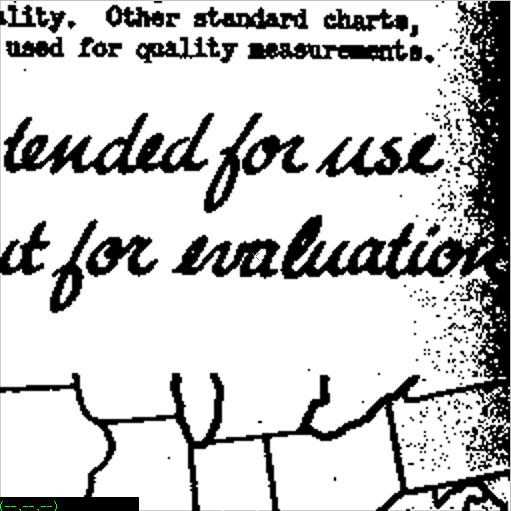
\includegraphics[width=3cm]{fac_d=5}
%\caption{fig1}
\end{minipage}%
}%
\subfigure[d=8.]{
\begin{minipage}[t]{0.25\linewidth}
\centering
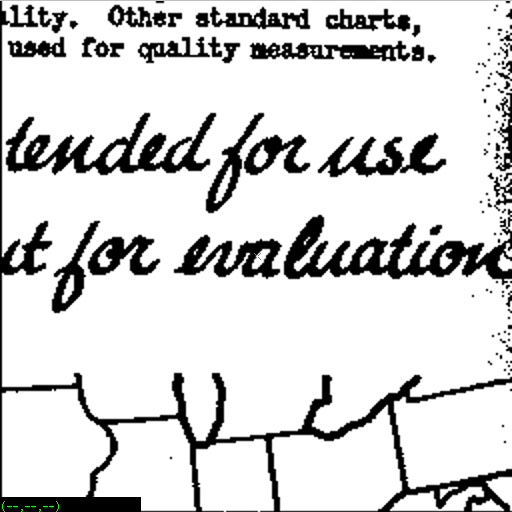
\includegraphics[width=3cm]{fac_d=8}
%\caption{fig2}
\end{minipage}%
}%

\subfigure[d=10.]{
\begin{minipage}[t]{0.25\linewidth}
\centering

\includegraphics[width=3cm]{fac_d=10}
%\caption{fig2}
\end{minipage}
}%
\centering
\caption{ Picture of facsimile}
\end{figure}

\begin{figure}[H]
\centering
\subfigure[d=10.]{
\begin{minipage}[t]{0.25\linewidth}
\centering

\includegraphics[width=3cm]{shtl_d=10}
%\caption{fig1}
\end{minipage}%
}%
\subfigure[d=20.]{
\begin{minipage}[t]{0.25\linewidth}
\centering

\includegraphics[width=3cm]{shtl_d=20}
%\caption{fig2}
\end{minipage}%
}%

\centering
\caption{ Picture of shtl}
\end{figure}

\newpage
\section*{Section3 Iterative Threshold Selection}
The algorithm uses a while loop with for loop in it, and the behind algorithm is relatively simple that it does require any complex operation or algorithm, it basically computes two average value of a picture which is divided into two parts: one part with the pixel value bigger than the threshold and the other with pixel value smaller than the threshold value.
\par
\vspace{3mm}
The code of vits.c:
\lstset{language=C}
\begin{lstlisting}

#include "VisXV4.h"          /* VisionX structure include file       */
#include "Vutil.h"           /* VisionX utility header files         */

VXparam_t par[] =            /* command line structure               */
{
{  "if=",   0,   " input file, vtpeak: threshold between hgram peaks"},
{  "of=",   0,   " output file "},
{  "d=",    0,   " min dist between hgram peaks (default 10)"},
{  "-v",    0,   "(verbose) print threshold information"},
{   0,      0,   0} /* list termination */
};
#define  IVAL   par[0].val
#define  OVAL   par[1].val
#define  DVAL   par[2].val
#define  VFLAG  par[3].val

main(argc, argv)
int argc;
char *argv[];
{

    Vfstruct (im);                 /* input image structure          */
    int y,x;                       /* index counters                 */
    int i;

    int hist[256];                 /* histogram bins                 */
    int thresh=10;                    /* threshold                      */
    int maxbin;                    /* maximum histogram bin          */
    int nxtbin;                    /* second maximum bin             */
    int minbin;                    /* minumim histogram bin          */
    int maxa, maxb;       /* second maximum bin above/below maxbin   */
    int dist;                   /* minimum distance between maxima   */
    unsigned int sum1=0;
    unsigned int sum2=0;
    unsigned int counter1=0;
    unsigned int counter2=0;
    int counter=0;		
    VXparse(&argc, &argv, par);    /* parse the command line         */

    dist = 10;                    /* default dist */
    if (DVAL) dist = atoi(DVAL);  /* if d= was specified, get value */
    if (dist < 0 || dist > 255) {
	fprintf(stderr, "d= must be between 0 and 255\nUsing d=10\n");
        dist = 10;
    }

    while ( Vfread( &im, IVAL) ) {
        if ( im.type != VX_PBYTE ) {
              fprintf (stderr, "error: image not byte type\n");
              exit (1);
        }

        /* clear the histogram */
        for (i = 0; i < 256; i++) hist[i] = 0;

        /* compute the histogram */
        for (y = im.ylo; y <= im.yhi; y++)
            for (x = im.xlo; x <= im.xhi; x++)
                 hist[im.u[y][x]]++;

         /* find maximum bin for the entire histogram */
         //maxbin = 0;
         //for (i = 0; i <= 255; i++)
         //    if (hist[i] > hist[maxbin]) maxbin = i;

	   /* compute the threshold */
	while(counter<20)
	{
             int i;
		for(i=0;i<=255;i++)
		{	
			if(i>thresh)
				{
				sum1=sum1+i;
				counter1=counter1+1;
				}			
			else
				{				
				sum2=sum2+i;
			      counter2=counter2+1;
                                }
//fprintf(stderr, "sum1 = %d\n", sum1);
		thresh=(sum1/counter1+sum2/counter2)/2;
		sum1=0;
		sum2=0;
		counter1=0;
		counter2=0;
		counter++;
              }

	}
        //if(VFLAG)
             fprintf(stderr, "thresh = %d\n",
                                  thresh);

        /* apply the threshold */
        for (y = im.ylo; y <= im.yhi; y++) {
            for (x = im.xlo; x <= im.xhi; x++) {
                 if (im.u[y][x] >= thresh) im.u[y][x] = 255;
                 else                      im.u[y][x] = 0;
            }
        }

        Vfwrite( &im, OVAL);
    } /* end of every frame section */
    exit(0);
}
\end{lstlisting}

\begin{figure}[H]
\centering
\subfigure[original]{
\begin{minipage}[t]{0.25\linewidth}
\centering
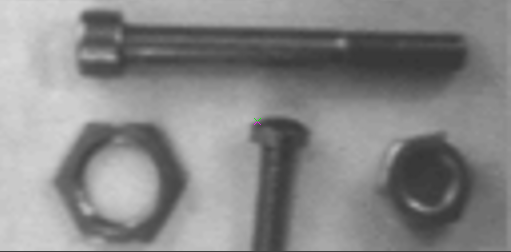
\includegraphics[width=3cm]{nb}
%\caption{fig1}
\end{minipage}%
}%
\subfigure[after thresholding]{
\begin{minipage}[t]{0.25\linewidth}
\centering

\includegraphics[width=3cm]{vits_nb}
%\caption{fig2}
\end{minipage}%
}%
\centering
\caption{ vits with small image}
\end{figure}

\begin{figure}[H]
\centering
\subfigure[original]{
\begin{minipage}[t]{0.25\linewidth}
\centering
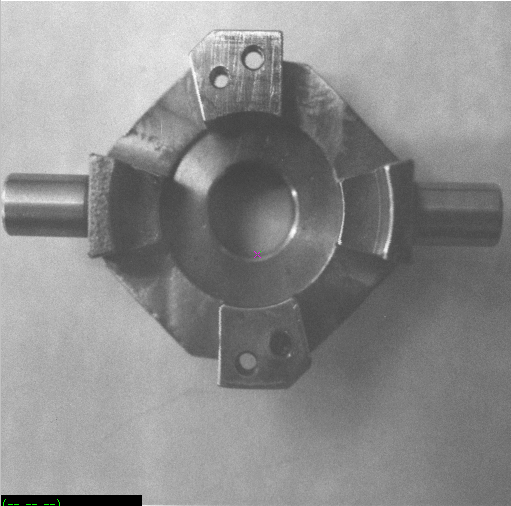
\includegraphics[width=3cm]{mp}
%\caption{fig1}
\end{minipage}%
}%
\subfigure[after thresholding]{
\begin{minipage}[t]{0.25\linewidth}
\centering
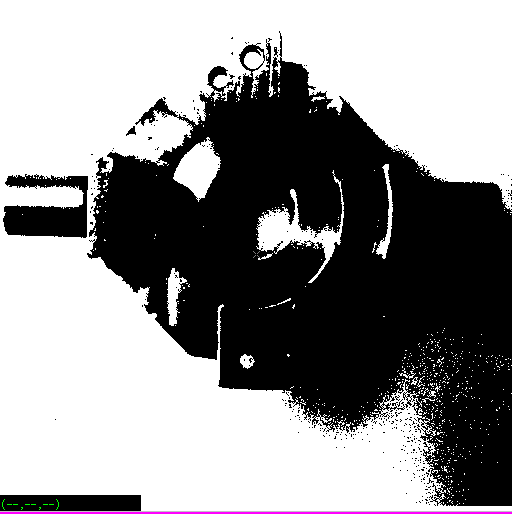
\includegraphics[width=3cm]{map_vits}
%\caption{fig2}
\end{minipage}%
}%
\centering
\caption{ vits with normal image}
\end{figure}



\newpage
\section*{Section4 Adaptive Thresholding}
thresholding is used to segment an image by setting all pixels whose intensity values are above a threshold to a foreground value and all the remaining pixels to a background value.
Whereas the conventional thresholding operator uses a global threshold for all pixels, adaptive thresholding changes the threshold dynamically over the image. This more sophisticated version of thresholding can accommodate changing lighting conditions in the image, e.g. those occurring as a result of a strong illumination gradient or shadows.
\begin{figure}[H]
\centering
\subfigure[original]{
\begin{minipage}[t]{0.25\linewidth}
\centering
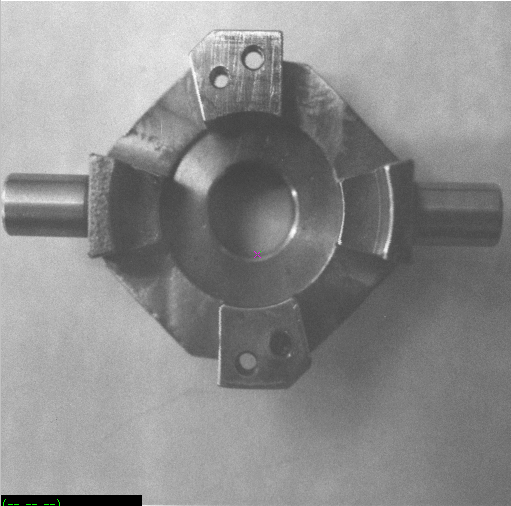
\includegraphics[width=3cm]{mp}
%\caption{fig1}
\end{minipage}%
}%
\subfigure[mp]{
\begin{minipage}[t]{0.25\linewidth}
\centering
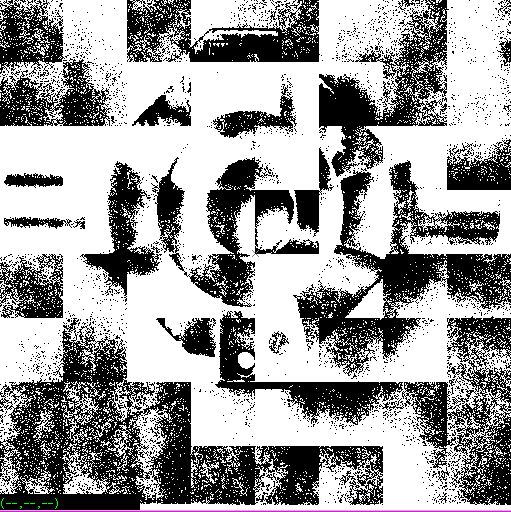
\includegraphics[width=3cm]{s4_mp}
%\caption{fig2}
\end{minipage}%
}%
\centering
\caption{ Adaptive thresholding}
\end{figure}
The best value found in the exmaple of mp.vx is: patch value:9, overlap value:8
\begin{figure}[H]
\centering
\subfigure[original]{
\begin{minipage}[t]{0.25\linewidth}
\centering
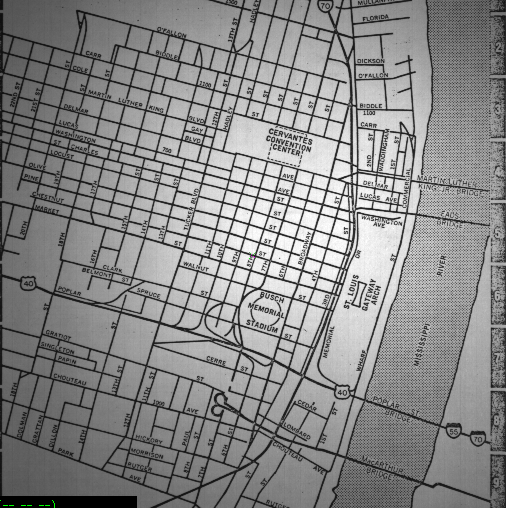
\includegraphics[width=3cm]{map}
%\caption{fig1}
\end{minipage}%
}%
\subfigure[mp.sq]{
\begin{minipage}[t]{0.25\linewidth}
\centering
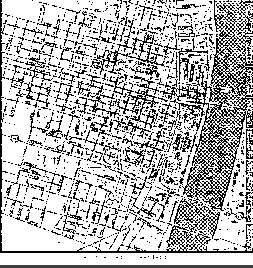
\includegraphics[width=3cm]{s4}
%\caption{fig2}
\end{minipage}%
}%
\centering
\caption{ Choosing the best value}
\end{figure}

\newpage
\section*{Section5 Region Growing}
\subsection*{5.1 Region growing on small images}
The program of region growing is mainly about recursive application, finding the condition to continue the region grow unless the conditions are not satisfied, then return. My program update the first pixel value in the iteration operation did on everyone pixel of the input image and then use recursive operation to update the label of the input image, which was done without redundant operation of coding and is pretty easy. When it comes to parser, I finish it by writing more parameters into the data structure in the vision called VXparam\_t.

\begin{figure}[h]
\centering
\subfigure[r=80]{
\begin{minipage}[t]{0.25\linewidth}
\centering
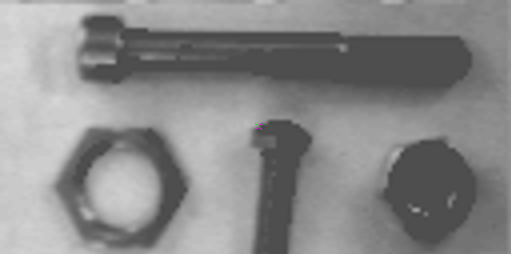
\includegraphics[width=3cm]{s5_80}
%\caption{fig1}
\end{minipage}%
}%
\subfigure[r=100]{
\begin{minipage}[t]{0.25\linewidth}
\centering
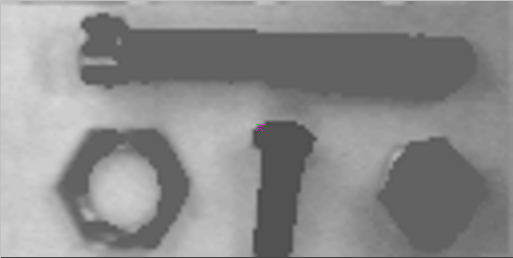
\includegraphics[width=3cm]{s5_100}
%\caption{fig2}
\end{minipage}%
}%

\subfigure[r=120]{
\begin{minipage}[t]{0.25\linewidth}
\centering
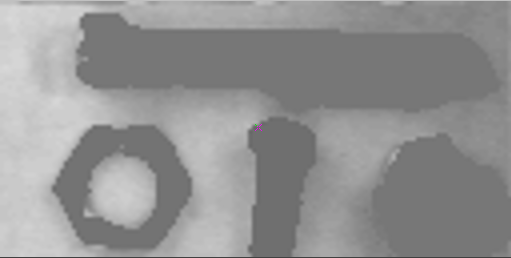
\includegraphics[width=3cm]{s5_120}
%\caption{fig2}
\end{minipage}
}%
\subfigure[r=150.]{
\begin{minipage}[t]{0.25\linewidth}
\centering

\includegraphics[width=3cm]{s5_150}
%\caption{fig2}
\end{minipage}
}%
\centering
\caption{ Region growing of nb.vx}
\end{figure}

\newpage
\subsection*{5.2 Region growing on image shtl.vx}
From the Figure below, we can easily get the best value r for different pictures and how the Adaptive Thresholding works in different pictures. For the shtl.vx image, due to the color of the background is not static and varies in a linear way, so when applying Adaptive Thresholding, you can see that the background of the image was divided into several different color parts, such as the picture when r=120 and r=140.
\begin{figure}[H]
\centering
\subfigure[original]{
\begin{minipage}[t]{0.25\linewidth}
\centering
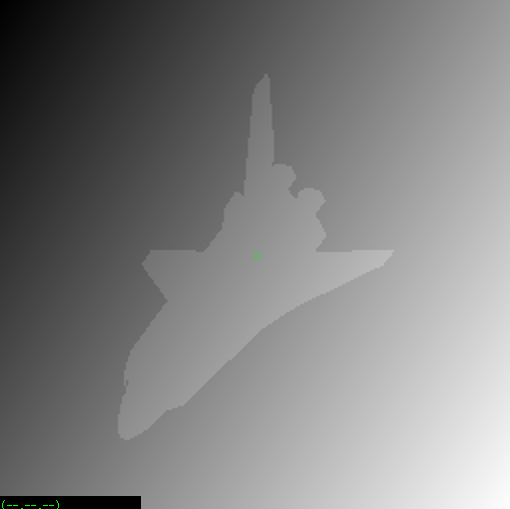
\includegraphics[width=3cm]{s5_shtl_original}
%\caption{fig1}
\end{minipage}%
}%
\subfigure[r=100]{
\begin{minipage}[t]{0.25\linewidth}
\centering
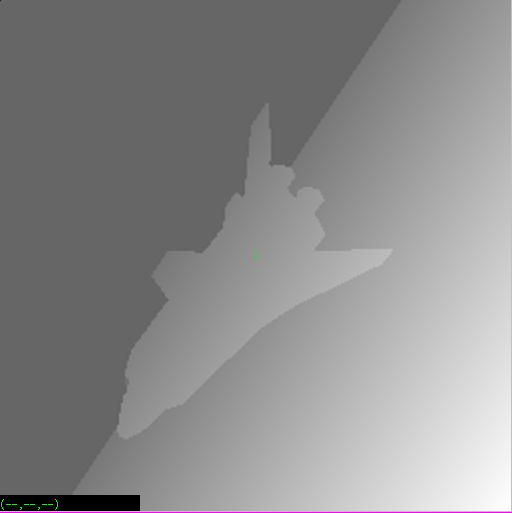
\includegraphics[width=3cm]{s5_shtl_100}
%\caption{fig2}
\end{minipage}%
}%

\subfigure[r=120]{
\begin{minipage}[t]{0.25\linewidth}
\centering
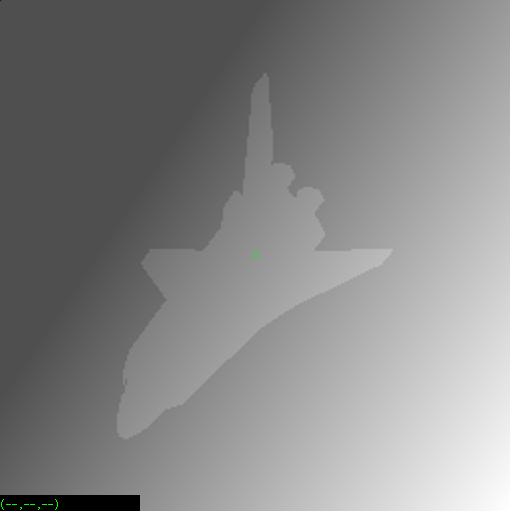
\includegraphics[width=3cm]{s5_shtl_120}
%\caption{fig2}
\end{minipage}
}%
\subfigure[r=140]{
\begin{minipage}[t]{0.25\linewidth}
\centering
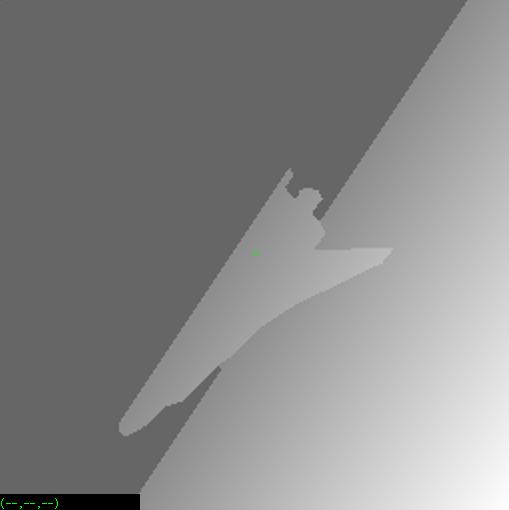
\includegraphics[width=3cm]{s5_shtl_140}
%\caption{fig2}
\end{minipage}
}%
\centering
\caption{ Region growing of shtl.vx}
\end{figure}


%----------------------------------------------------------------------------------------
%	BIBLIOGRAPHY
%----------------------------------------------------------------------------------------

%\bibliographystyle{apalike}

%\bibliography{sample}

%----------------------------------------------------------------------------------------


\end{document}
